\documentclass[11pt,a4paper]{article}
\usepackage[a4paper,margin=2.2cm]{geometry}
\usepackage[T1]{fontenc}
\usepackage{lmodern}
\usepackage{microtype}
\usepackage{graphicx}
\usepackage{enumitem}

\pagestyle{empty}
\setlist{itemsep=2pt,topsep=3pt,leftmargin=1.4em}
\setlength{\parskip}{5pt}

\begin{document}

\begin{center}
  {\LARGE\bfseries M1 Report}\\[6pt]
  {\large Team 82}
\end{center}
\vspace{4pt}

\section{Problem Statement and Understanding}

The problem statement, \emph{Empowering the Next Generation Through Financial Literacy}, asks for a scalable way to teach money skills to Grade 11--12 students (ages 16--18) in Hyderabad, delivered through NGO partners to a pilot of about 1,500 students. It covers five areas: opening a bank account and using digital payments, budgeting, saving and borrowing, the basics of investing, and staying safe from fraud.

Our reading of the problem is that money lessons rarely stick when they are taught as rules. Students learn ``keep an emergency fund'' or ``never share your PIN'', but never feel what happens when they ignore it, and in real life the consequences arrive weeks later and are too costly to learn from. The solution also has to work in a difficult setting: low-end and often shared phones, unreliable internet in classrooms, several languages (English, Telugu, Hindi, Urdu), and facilitators who need to see where a class is struggling. Because the users are minors, it must not collect real financial or family data, and it must educate without recommending any real investment product.

\section{Idea}

We are building a \textbf{financial life simulator} rather than a course. A student first creates a fictional character by answering ten short picture-based questions (age, source of income, household, goal and attitude to money). They then live that character's financial year month by month, starting from opening a bank account and moving through seven stages: getting banked, digital payments, a first budget, saving and tracking, borrowing decisions, growing money, and protecting it.

Mistakes are safe. The character can overspend, fall for a simulated scam or miss a goal, and the student can then \textbf{rewind} to an earlier decision, choose differently, and compare the two lives side by side. Both timelines share the same random events, so any difference comes from the decision and not from luck.

Around this main mode sit short mini-games for focused practice (for example a bank counter, a budgeting jar split, a stock market with fictional companies, a scam inbox), a library of quick scenarios with a daily challenge, and a dashboard where facilitators create classes, unlock stages and see which concepts their students find difficult.

\section{Approach and Architecture}

The app is an offline-first progressive web app. All game logic lives in a pure TypeScript core that is separate from the interface, and all scenarios are stored as JSON content so that new ones can be added without code changes.

\begin{center}
  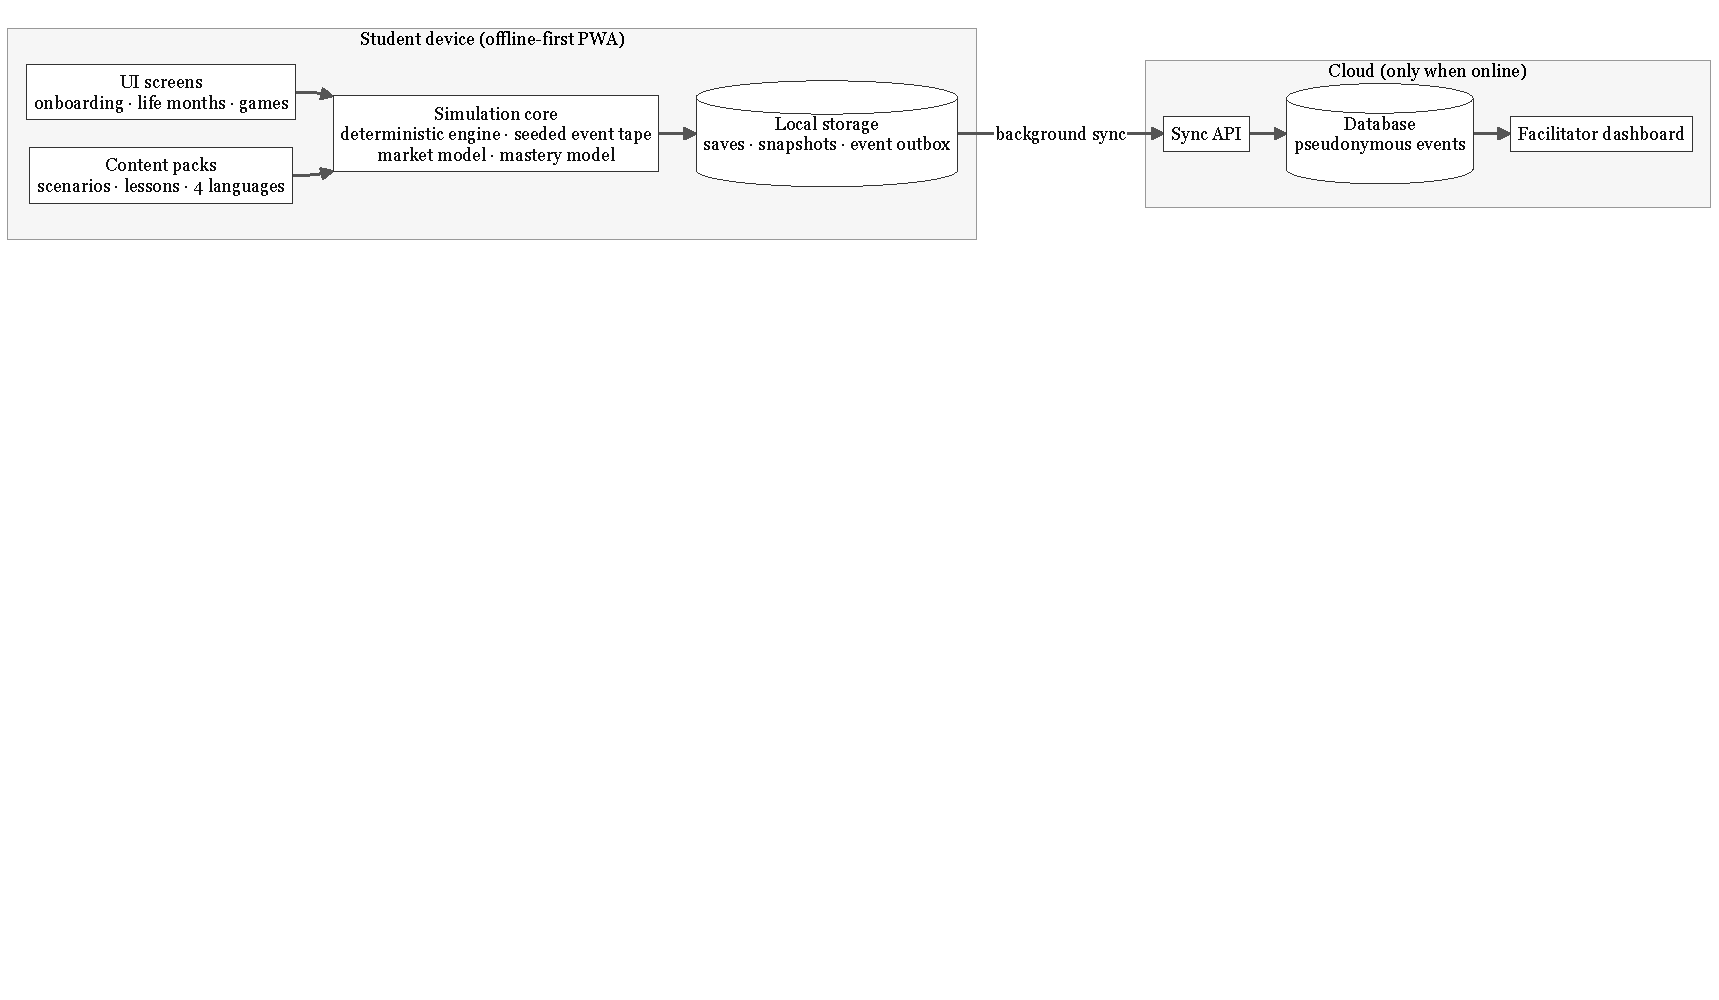
\includegraphics[width=\linewidth,trim=0 345 0 0,clip]{arch_raw.pdf}
\end{center}

\begin{itemize}
  \item \textbf{Deterministic engine.} The simulation is a pure function from state and action to the next state. Random events (price shocks, festivals, scam messages, market moves) come from a seeded event tape, so the same seed and the same choices always produce the same result. This is what makes rewind, fair comparison and testing possible.
  \item \textbf{One learning loop.} Every activity follows the same steps: a short story, the decision or game, the consequence, a ``why did this happen?'' question that detects misconceptions, the concept, an optional retry, two or three check questions, and a reward.
  \item \textbf{Mastery tracking.} Each concept has a mastery value between 0 and 1 that moves towards the correctness of each answer. Weak concepts return later as review questions.
  \item \textbf{Privacy and guardrails.} Students sign in with a class code and a picture PIN, with no email or phone number. Only pseudonymous gameplay events are synced. Investing screens use fictional assets only and show results as ranges under stated assumptions.
\end{itemize}

The stack is React, TypeScript and Tailwind on the client, IndexedDB for local storage, and Supabase (PostgreSQL with row-level security) for classes and synced events. The project scaffold, student setup flow, facilitator dashboard, local storage with sync outbox, market simulation and the first investing lessons are already in place, with 143 passing unit tests.

\section{Testing Methodology}

\begin{itemize}
  \item \textbf{Unit tests.} Since the core is made of pure functions, the engine, financial calculations, market model and mastery updates are tested directly with Vitest in continuous integration. The character builder is tested over every possible combination of answers.
  \item \textbf{Determinism and rewind.} We check that the same seed and choices give identical saved state, that random events fall in the same month in both timelines after a rewind, and that the original timeline is never modified.
  \item \textbf{Content checks.} A schema validator checks every scenario for missing text, concepts or translations, and a word-list test fails the build if a real bank, fund or company name appears.
  \item \textbf{Simulation checks.} Simulated returns are compared with closed-form expectations, and running 500 simulated futures must take under one second on a low-end phone.
  \item \textbf{Device tests.} Each screen is checked on a 360\,$\times$\,640 display, with large text and right-to-left Urdu, and the app is played in airplane mode and then reconnected to confirm that data syncs.
  \item \textbf{Learning gain.} A short pre-check and post-check drawn from separate question pools measure improvement on unseen questions. We will also run quick playtests with peers and time each module.
\end{itemize}

\end{document}
